%! TEX root = Geometria.tex

\documentclass{./Geometria.tex}
\begin{document}
\chapter{Espacio Afín}
\section{El espacio afín}
Dados un conjunto de elementos, siendo estos puntos, $A$, y un espacio vectorial $\mathbb{V}$, llamamos el espacio afín a la terna $(A,\mathbb{V},\varphi)$, siendo $\varphi$ una aplicación entre elementos de $A$, tal que:
$$
\varphi: A \times A \mapsto \mathbb{V}
$$
Esta terna debe cumplir que:
\begin{itemize}
    \item $\forall p \in A \wedge \mathbf{v} \in \mathbb{V}, \exists! Q \in A/ \varphi(P,Q) = \mathbf{PQ}=\mathbf{u}=Q-P$
    \item Relaci\'on de Chasles: $\forall P,Q,R \in A \wedge\varphi (P,Q) + \varphi (Q,R) = \varphi (P,R)$
\end{itemize}
$$
\mathbf{PQ} + \mathbf{QR} = \mathbf{PR}
$$

\textbf{Demostraci\'on}
\begin{itemize}
    \item $\mathbf{PQ}=Q-P$
    \item $\mathbf{QR}=R-Q$ 
\end{itemize}
$$
\mathbf{PQ}+\mathbf{QR} = Q-P +R-Q = R-P = \mathbf{PR} 
$$
La dimensi\'on del espacio af\'in va a ser la dimensi\'on de $\mathbb{V}$. 

\section{Propiedades del espacio af\'in}
\begin{itemize}
    \item $\forall P \in A, \varphi(P,P)=0$
    \item $\varphi(P,Q)=0 \iff P=Q$
    \item $\forall P,Q \in A, \varphi(P,Q) = -\varphi(Q,P)$
    \item Regla del paralelogramo: $\forall P,Q,R,S \in A$:
$$
\varphi(P,Q)=\varphi(R,S) \iff \varphi (P,R) = \varphi (Q,S)
$$
\end{itemize}

\section{Vector de posici\'on}
Es un vector que representa la posici\'on de un punto en el espacio respecto a un origen, adem\'as de la distancia que separa dichos puntos. El vector $\mathbf{OP}$ es el vector que une el origen al punto $P$. Esta aplicaci\'on es \textbf{biyectiva} (inyectiva y sobreyectiva).

\begin{defin}
Supongamos que no es inyectiva. Es decir, existen dos $\varphi(x)=\varphi (y) / x \neq y$ 
\begin{equation}
	\begin{split}		
		\mathbf{OP}+\mathbf{PQ}&=\mathbf{OQ} \\
		\mathbf{P}+\mathbf{PQ}&=\mathbf{Q} \\
		\mathbf{P}=\mathbf{Q} &\implies \mathbf{OP}=\mathbf{OQ} \\
		&\implies P = Q
	\end{split}
\end{equation}
\end{defin}

\section{Estructura af\'in can\'onica}
Dado un espacio vectorial $\mathbb{V}$, la aplicaci\'on $\varphi$
$$
\varphi: \mathbb{V} \times \mathbb{V} \to \mathbb{V}; \mathbf{uv}=\mathbf{v}-\mathbf{u}
$$
satisface los axiomas de la definici\'on de un espacio af\'in y define una estructura de espacio af\'in $(\mathbb{V}, \mathbb{V}, \varphi)$ conocida como la estructura af\'in can\'onica de $\mathbb{V}$.

\section{Traslaci\'on de un vector}
Dado $\mathbf{v}\in \mathbb{V}$, la traslaci\'on de un vector es la aplicaci\'on
$$
\tau_{\mathbf{v}}: A \to A
$$
$$
\tau_{\mathbf{v}} (P)=P+\mathbf{v}=Q
$$
Una traslaci\'on de vector $\mathbf{v}$ transforma el punto $P$ a otro punto $Q$.

\subsection{Propiedades de traslaci\'on}
\begin{itemize}
    \item $\tau_{\mathbf{0}}(P)=P$
    \item $\tau_{\mathbf{u}} \circ \tau_{\mathbf{v}}=\tau_{\mathbf{v}} \circ\tau_{\mathbf{u}}=\tau_{\mathbf{u}+\mathbf{v}}$
\end{itemize}

\begin{teorema}
Cualquier transformación afín se puede escribir como un producto de una transformación afín.
\end{teorema}

\section{Suma de un punto y un vector}
Fijado $P \in A$, denotaremos por $F_{P}: A \to \mathbf{A}$ a la aplicaci\'on dada por $F_{P}(Q)=\mathbf{PQ}$. Si $P \in A$ y $\mathbf{v}\in A$, el \'unico punto $Q\in A$ dado, tal que $\mathbf{PQ}=\mathbf{v}$ se denotar\'a como $P+\mathbf{v}$.

\begin{teorema}
Dados un espacio af\'in y una transformaci\'on af\'in $f:A \to A$. Entonces son equivalentes:
\begin{itemize}
    \item Existe un conjunto fijo $V$ no trivial $(V \neq \{ 0 \})$.
    \item El $1$ es autovalor de $f$.
\end{itemize}
El conjunto de puntos fijos es un subespacio af\'in de $A$ con subespacio vectorial asociado de $V$ de autovectores de $\bar{f}$ con autovalor $\lambda=1$.
\end{teorema}
\section{Teoremas adicionales}
\begin{teorema}
Dado un triángulo y sus \textbf{cevianas} (rectas que parten de un vértice en intersecan el cateto opuesto), estas son concurrentes si y solo si:
\begin{equation}
	\begin{split}
		\frac{a}{b} \frac{c}{d} \frac{e}{f} = 1
	\end{split}
\end{equation}
El caso mostrado en la figura \ref{fig:ceva} es un casto donde el teorema aplica.
\end{teorema}
\begin{figure}[ht]
	\centering


\tikzset{every picture/.style={line width=0.75pt}} %set default line width to 0.75pt

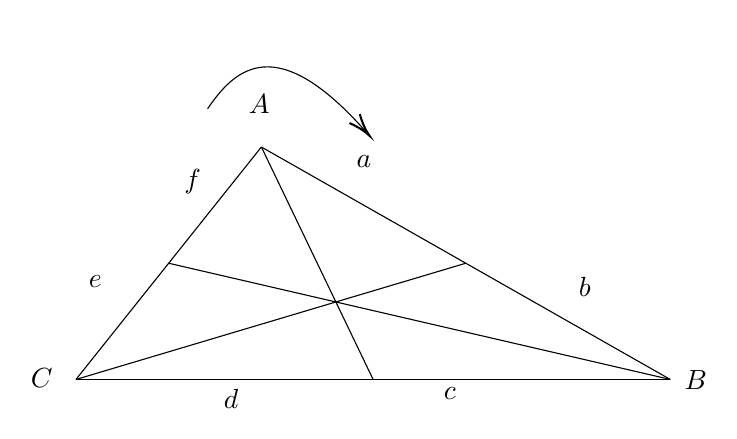
\begin{tikzpicture}[x=0.75pt,y=0.75pt,yscale=-1,xscale=1]
%uncomment if require: \path (0,300); %set diagram left start at 0, and has height of 300

%Straight Lines [id:da6088495384470597]
\draw    (159,213.7) -- (445.33,213.7) ;
%Straight Lines [id:da9392487083542241]
\draw    (159,213.7) -- (248.33,101.7) ;
%Straight Lines [id:da109210029532397]
\draw    (248.33,101.7) -- (445.33,213.7) ;
%Straight Lines [id:da003882238193997689]
\draw    (248.33,101.7) -- (302.17,213.7) ;
%Straight Lines [id:da19764114058099969]
\draw    (159,213.7) -- (346.83,157.7) ;
%Straight Lines [id:da40447162391369784]
\draw    (445.33,213.7) -- (203.67,157.7) ;
%Curve Lines [id:da25395723032690765]
\draw    (222.42,83.28) .. controls (235.35,64.38) and (255.22,44.48) .. (299.74,95.51) ;
\draw [shift={(300.42,96.28)}, rotate = 229.13] [color={rgb, 255:red, 0; green, 0; blue, 0 }  ][line width=0.75]    (10.93,-3.29) .. controls (6.95,-1.4) and (3.31,-0.3) .. (0,0) .. controls (3.31,0.3) and (6.95,1.4) .. (10.93,3.29)   ;

% Text Node
\draw (241,75.4) node [anchor=north west][inner sep=0.75pt]    {$A$};
% Text Node
\draw (451,208.4) node [anchor=north west][inner sep=0.75pt]    {$B$};
% Text Node
\draw (136,207.4) node [anchor=north west][inner sep=0.75pt]    {$C$};
% Text Node
\draw (293,104.4) node [anchor=north west][inner sep=0.75pt]    {$a$};
% Text Node
\draw (400,163.4) node [anchor=north west][inner sep=0.75pt]    {$b$};
% Text Node
\draw (335,216.4) node [anchor=north west][inner sep=0.75pt]    {$c$};
% Text Node
\draw (229,217.4) node [anchor=north west][inner sep=0.75pt]    {$d$};
% Text Node
\draw (164,162.4) node [anchor=north west][inner sep=0.75pt]    {$e$};
% Text Node
\draw (210,111.4) node [anchor=north west][inner sep=0.75pt]    {$f$};


\end{tikzpicture}

\caption{Teorema de Ceva}
\label{fig:ceva}
\end{figure}
\begin{teorema}
	Dado un triángulo, los puntos $D, E, F$ están en la misma línea sí y solo si:  
	\begin{equation}
		\begin{split}
			\frac{AD}{DB} \frac{BE}{EC} \frac{CF}{FA}
		\end{split}
	\end{equation}
	Como se ve en la figura \ref{fig:menelao}.
\end{teorema}
\begin{figure}
	\centering


\tikzset{every picture/.style={line width=0.75pt}} %set default line width to 0.75pt

\begin{tikzpicture}[x=0.75pt,y=0.75pt,yscale=-1,xscale=1]
%uncomment if require: \path (0,300); %set diagram left start at 0, and has height of 300

%Straight Lines [id:da17874017551751153]
\draw    (132,202.33) -- (234.33,63.33) ;
%Straight Lines [id:da7098324394058902]
\draw    (234.33,63.33) -- (364.42,202.08) ;
%Straight Lines [id:da5613310647299824]
\draw    (132,202.33) -- (364.42,202.08) ;
%Straight Lines [id:da5056130723161624]
\draw  [dash pattern={on 4.5pt off 4.5pt}]  (364.42,202.08) -- (554.58,202.08) ;
%Straight Lines [id:da8097180730683872]
\draw    (199.42,111.58) -- (478.42,200.58) ;

% Text Node
\draw (118,206.4) node [anchor=north west][inner sep=0.75pt]    {$A$};
% Text Node
\draw (229,40.4) node [anchor=north west][inner sep=0.75pt]    {$B$};
% Text Node
\draw (365,214.4) node [anchor=north west][inner sep=0.75pt]    {$C$};
% Text Node
\draw (176,91.4) node [anchor=north west][inner sep=0.75pt]    {$D$};
% Text Node
\draw (320,126.4) node [anchor=north west][inner sep=0.75pt]    {$E$};
% Text Node
\draw (484,210.4) node [anchor=north west][inner sep=0.75pt]    {$F$};


\end{tikzpicture}
\caption{Teorema de Menelao}
\label{fig:menelao}
\end{figure}
\end{document}

